\documentclass{beamer}

\title{Confidence Distributions in Meta-Analysis}
\subtitle{Student Research Conference, BYU}
\author{Travis Andersen \\ Dr Brinley Zabriskie}

% Questions:
% Standard errors are articially small when normality is assumed
% P-value function is a subset of confidence distribution
% Verbally say why second point of last slide is useful
%   One good thing is eliminating upper limit going to infinity

% To do:
% Change Norris to 10 and 15, first Kahler to 0
% Look up beta blockers: reduce blood pressure
% Maybe get rid of inference slide 2
% Increase size of labels on confidence intervals plot


\begin{document}

\begin{frame}
  \maketitle
\end{frame}

%%%%%%%%%%%%%%%%%%%% Statistical Inference %%%%%%%%%%%%%%%%%%%%
\begin{frame}
  \frametitle{Statistical inference}
  \begin{table}
  \begin{tabular}{| c | c | c |} \hline
    Group & Event & No Event \\ \hline
    Treatment & 10 & 42 \\ \hline
    Control & 12 & 35 \\ \hline
  \end{tabular}
  \end{table}
  \begin{equation*}
    \text{Odds Ratio} = \frac{\text{ET}/\text{NT}}{\text{EC}/\text{NC}}
  \end{equation*}
  \begin{equation*}
    \hat{\text{OR}} = 0.694, \, 
    \text{P-value} = 0.453, \,
    \text{95\% CI} = (0.268, 1.80)
  \end{equation*}
\end{frame}

\begin{frame}
  \frametitle{Statistical inference}
  \begin{itemize}
    \item We are interested in $\theta$
    \item P-values: $P(\text{abs}(T) \geq \text{abs}(t)|\theta = \theta_0)$
    \item Confidence intervals: $\hat{\theta} \pm z^*(\alpha) \text{SE}(\hat{\theta})$
  \end{itemize}
\end{frame}

\begin{frame}
  \frametitle{Statistical Inference}
  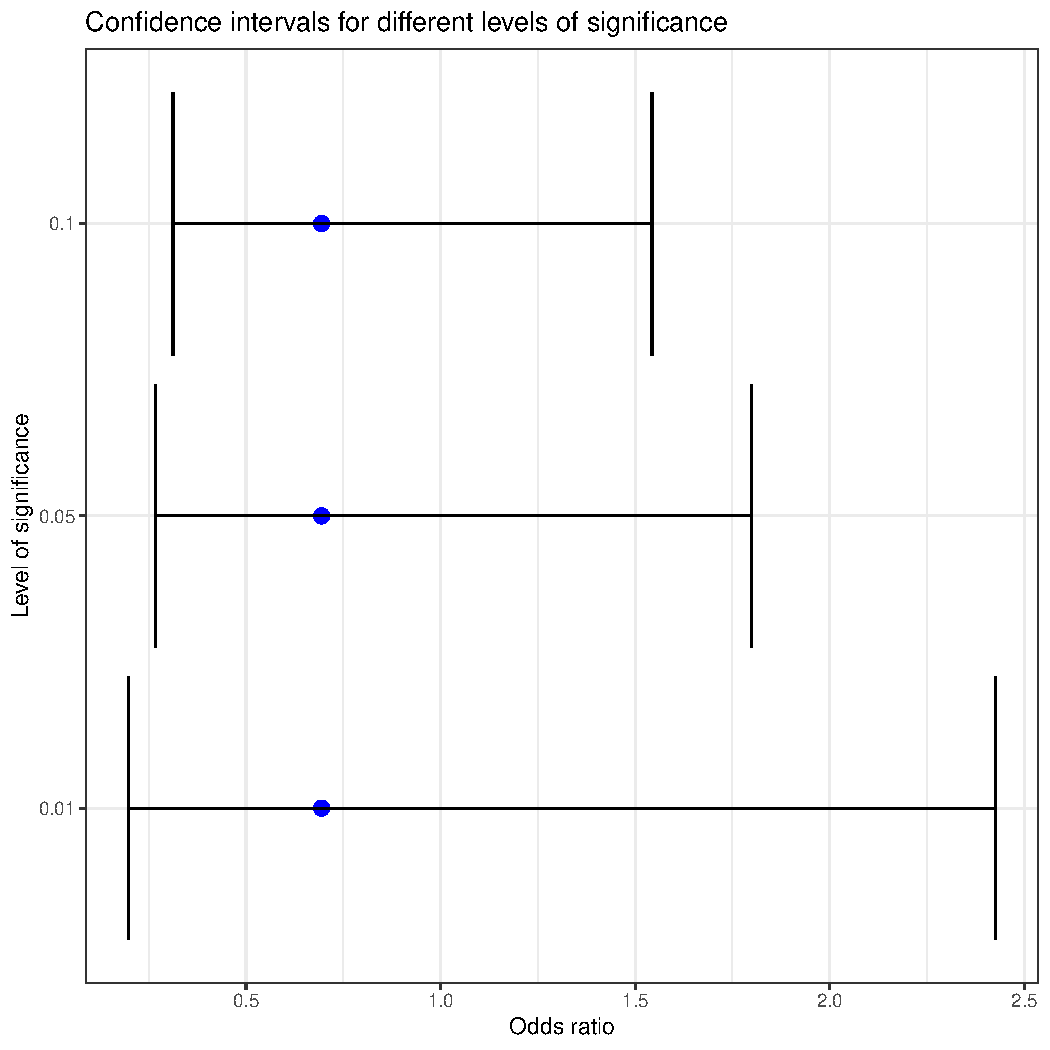
\includegraphics[scale = 0.4]{cis}
 
  Inference depends on choice of level of significance and null value
\end{frame}

%%%%%%%%%%%%%%%%%%%% P-value functions %%%%%%%%%%%%%%%%%%%%
\begin{frame}
  \frametitle{P-value functions}
  \begin{itemize}
    \item Compute p-values for all levels of significance
    \item Allows for field experts to make decision
  \end{itemize}
\end{frame}

\begin{frame}
  \frametitle{P-value functions}
  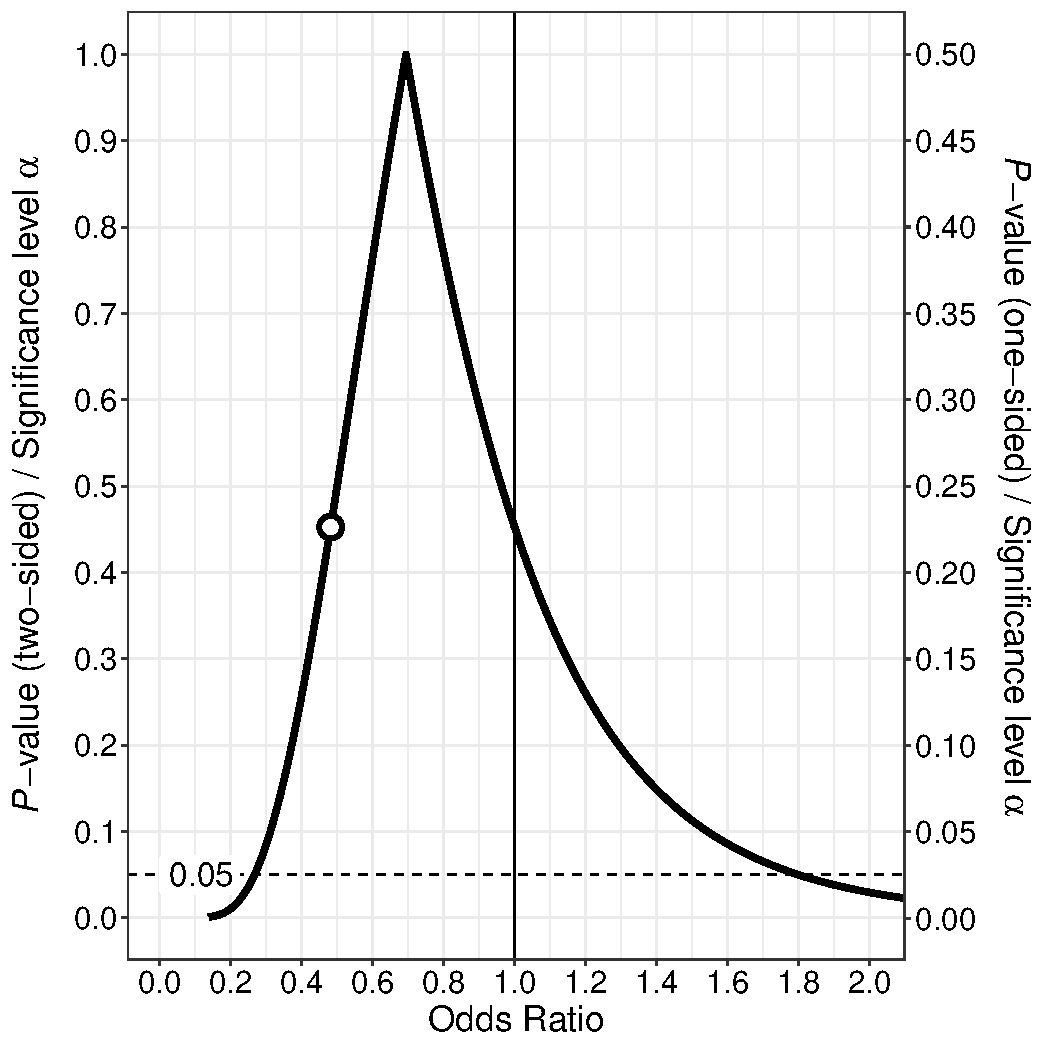
\includegraphics[scale = 0.45]{cd1}
\end{frame}

\begin{frame}
  \frametitle{P-value functions}
  \begin{equation*}
    \alpha = 2\left(1 - \Phi \left(\frac{|\theta - \hat{\theta}|}{\text{SE}(\hat{\theta})}\right) \right)
  \end{equation*}
  \begin{itemize}
    \item $\alpha$: level of significance
    \item $\theta$: parameter of interest
    \item $\hat{\theta}$: estimate of $\theta$
    \item $\Phi$: standard normal cdf
  \end{itemize}
\end{frame}

%%%%%%%%%%%%%%%%%%%% Meta-Analysis %%%%%%%%%%%%%%%%%%%%
\begin{frame}
  \frametitle{Meta-Analysis}
  \begin{tabular}{|c | c | c | c | c|}
    \hline
    Author & Ee & Ne & Ec & Nc \\ 
    \hline
    Barber & 10 & 42 & 12 & 35 \\
    Norris & 5 & 221 & 15 & 213 \\
    Kahler & 0 & 38 & 6 & 25 \\
    Ledwich & 2 & 18 & 3 & 17 \\
    \hline
  \end{tabular}
\end{frame}

\begin{frame}
  \frametitle{Meta-Analysis}
  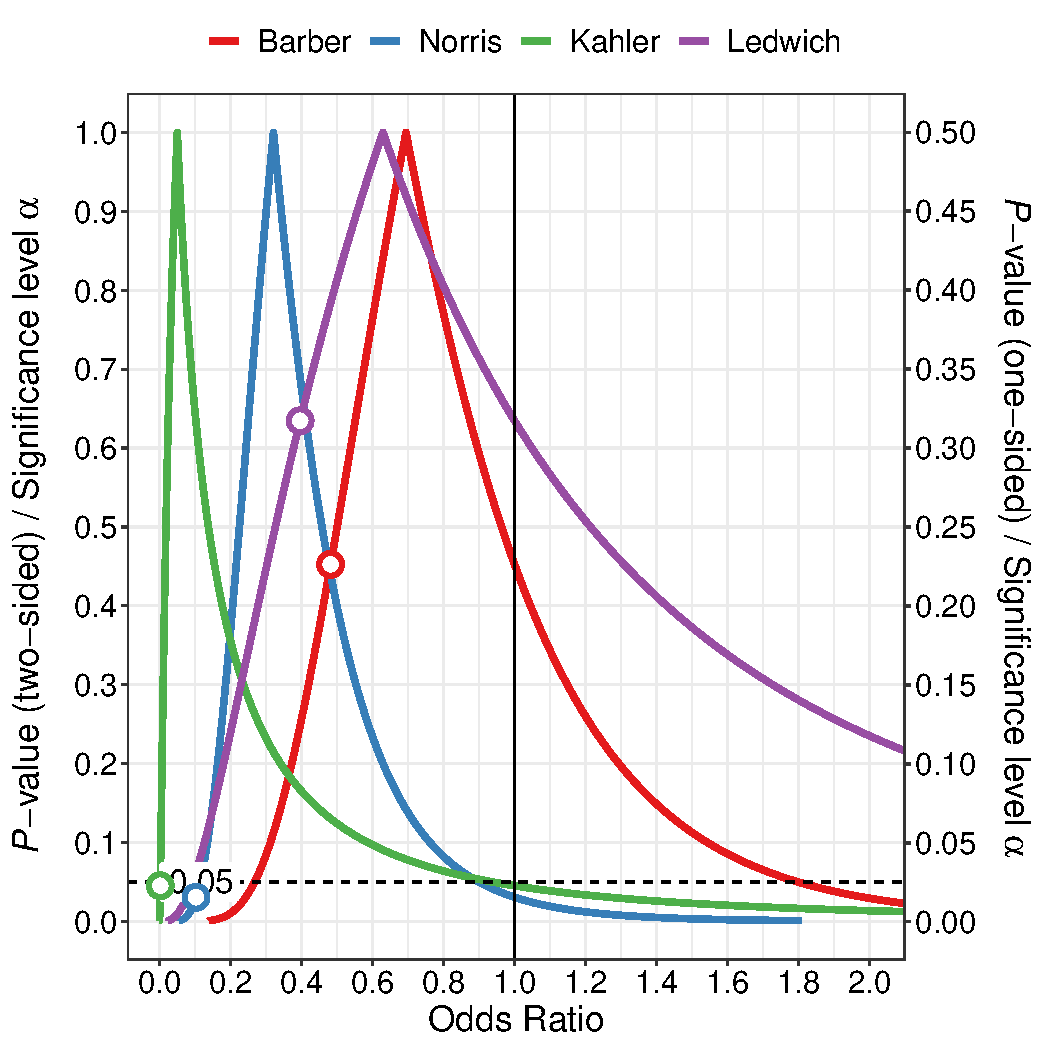
\includegraphics[scale = 0.45]{cd3}
\end{frame}

\begin{frame}
  \frametitle{Meta-Analysis}
  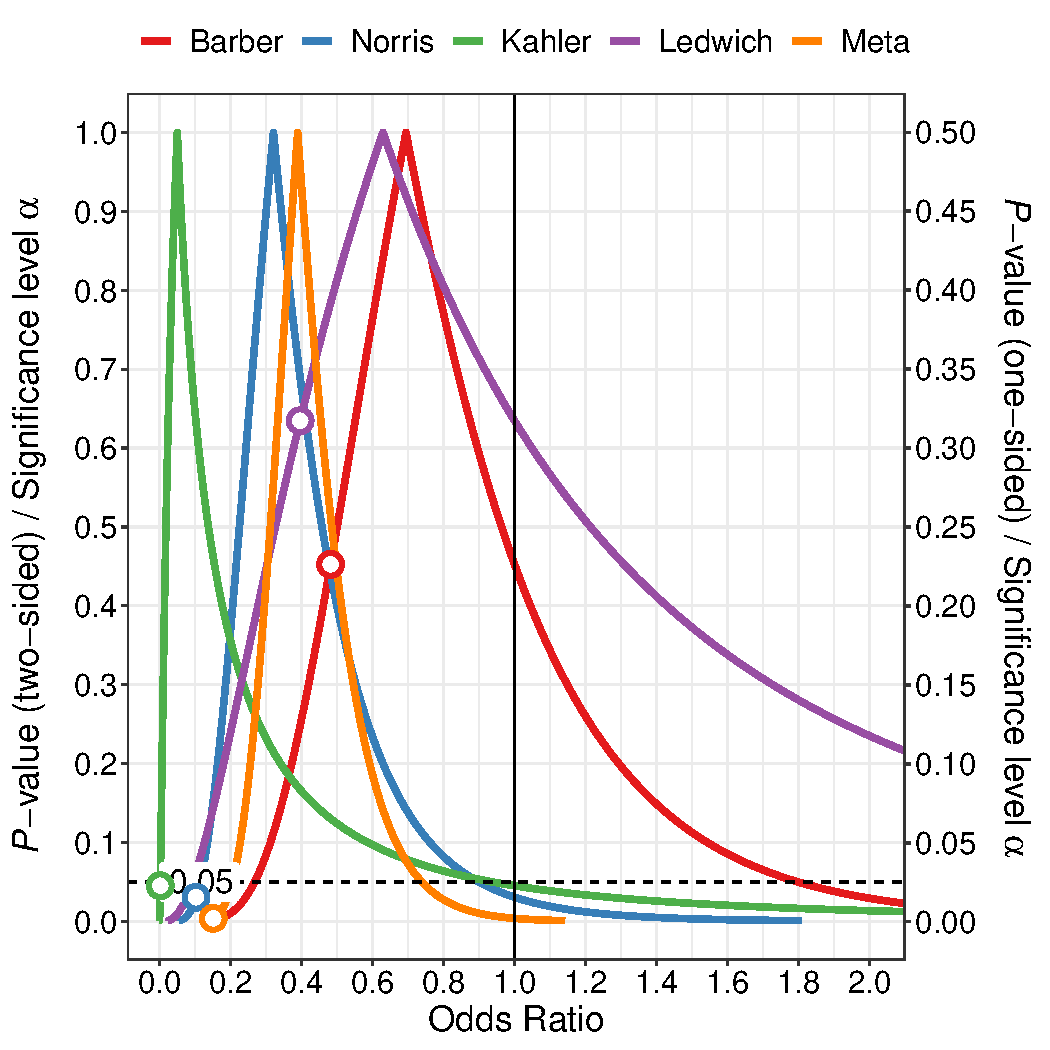
\includegraphics[scale = 0.45]{cd_meta}
\end{frame}

\begin{frame}
  \frametitle{Meta-Analysis}
  \begin{itemize}
    \item In approaches above, normality is assumed
    \item Goal: create an exact confidence distribution for rare event meta-analyses
  \end{itemize}
\end{frame}

\end{document}